\section{Auswahl der Daten}
\subsection{Reineke-Gleichung}
\begin{frame}[c]
  \visible<\theFirstElement->{
    \begin{center}
      \begin{minipage}{0.40\textwidth}
        \centerline{\(\mylog(N) = \textcolor{red}{s} \log(D) + k\)}
        \vspace{\captiondistance}
        \mycaption{Gleichung 1}{Bestandesdichte in Abhängigkeit von mittlerem Durchmesser (Quelle: [1]). \\
          \(N\): Bestandesdichte [\si{\per\hectare}] \\
          \(s\): \textcolor{red}{Steigung} \\
          \(D\): Durchmesser des Grundflächenmittelstammes [\si{\centi\meter}] \\
          \(k\): Konstante (artabhängig)}
      \end{minipage}
    \end{center}

    % \begin{align*}
      % \myscalebox{N} & \myscalebox{: \text{Bestandesdichte [ha\textsuperscript{-1}]}} \\[-3mm]
      % \myscalebox{s} & \myscalebox{: \text{Steigung (}\widehat{=}\text{ \textcolor{red}{Mortalitätsrate})}} \\[-3mm]
      % \myscalebox{D} & \myscalebox{: \text{Durchmesser des Grundflächemittelstammes [cm]}} \\[-3mm]
      % \myscalebox{k} & \myscalebox{: \text{Konstante (artabhängig)}} \\[-3mm]
    % \end{align*}
  }

  \begin{itemize}
  \item<\theSecondElement-> Literatur: \\
    Steigung scheint art- und standortabhängig zu sein (s. z.B. [2])
  \item<\theSecondElement-> Lösungsansatz: \\
    artabhängiger Korridor ,,erlaubter`` Steigungen, begrenzt durch unteren Schwellwert (\(m_u\)) und oberen Schwellwert (\(m_o\))
  \end{itemize}
\end{frame}

\subsection{Auswahlmechanismus}
\begin{frame}[c]
  \begin{columns}
    \begin{column}{0.5\textwidth}
      \visible<\theFirstElement->{
        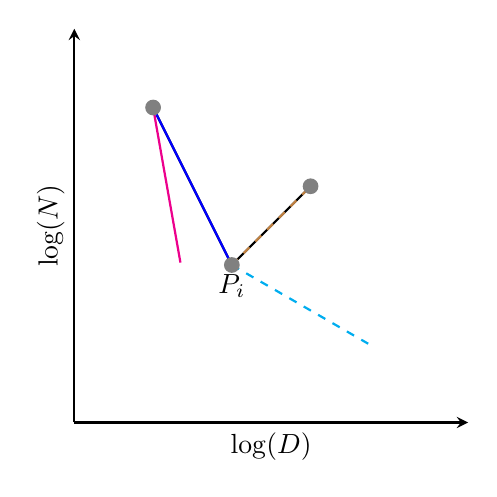
\begin{tikzpicture}[>=stealth]
          %% Coordinate system.
          \draw[black,thick,->] (0,0) -- (5,0);  %% x-axis
          \draw[black,thick,->] (0,0) -- (0,5);  %% y-axis
          \node[anchor=north] at (2.5,0) {\(\log(D)\)};  %% x-axis title
          \node[anchor=south,rotate=90] at (0,2.5) {\(\log(N)\)};  %% y-axis title
          
          %% Specify point coordinates.
          \coordinate (Pi-1) at (1,4);
          \coordinate (Pi) at (2,2);
          \coordinate (Pi+1) at (3,3);

          %% Lines.
          \visible<\theFirstElement-\theSecondElement>{\draw[black,thick] (Pi-1) -- (Pi) -- (Pi+1);}
          \visible<\theSecondElement->{\draw[magenta,thick] (Pi-1) -- ++(280:2cm);}
          \visible<\theSecondElement->{\draw[blue,thick] (Pi-1) -- (Pi);}
          \visible<\theThirdElement->{\draw[cyan,thick,dashed] (Pi) -- ++(330:2cm);}
          \visible<\theThirdElement->{\draw[brown,thick,dashed] (Pi) -- (Pi+1);}

          %% Points.
          \fill[gray] (Pi-1) circle (0.1);
          \fill[gray] (Pi) circle (0.1);
          \fill[gray] (Pi+1) circle (0.1);

          %% Text.
          % \node[anchor=south] at (Pi-1) {\(\text{P}_{i-1}\)};
          \node[anchor=north] at (Pi) {\(\text{P}_i\)};
          % \node[anchor=south] at (Pi+1) {\(\text{P}_{i+1}\)};

        \end{tikzpicture}
        \captionsep{}
        \mycaption{Abbildung 1}{Schematische Darstellung der Funktionsweise des Auswahlmechanismus.}
      }
    \end{column}
    \begin{column}{0.5\textwidth}
      \visible<\theFirstElement->{\(\text{P}_i\) wird ausgewählt, wenn}
      \begin{enumerate}
      \item<\theFirstElement-> es mind. einen benachbarten Punkt gibt (\ding{51}) und
      \item<\theSecondElement-> Steigung \(\textcolor{blue}{s_1} \geq \textcolor{magenta}{m_u}\) (\ding{51}) und
      \item<\theThirdElement-> Steigung \(\textcolor{brown}{s_2} \leq \textcolor{cyan}{m_o}\) (\ding{55}).
      \end{enumerate}
    \end{column}
  \end{columns}
\end{frame}

\subsection{Beispiel: Buche}
\begin{frame}[c]
  \visible<1->{
    \centerline{
      \begin{minipage}{0.9\textwidth}
        \includegraphics[width=1.0\textwidth]{../../Graphics/Presentation/logDlogNPlotsBeforeAfterDataSelectionBeech.pdf}
        \captionsep{}
        \mycaption{Abbildung 2}{Beobachteter Zusammenhang zwischen Bestandesdichte \(N\) und mittlerem Durchmesser \(D\).  Farbige Linien verbinden Beobachtungen eines Bestandes. Gestrichelte bzw. durchgezogene schwarze Linien stellen den oberen bzw. unteren Schwellwert der noch ,,erlaubten`` Steigungen beispielhaft dar. \\
          A: vor Anwendung des Auswahlmechanismus \\
          B: nach Anwendung des Auswahlmechanismus}
      \end{minipage}}}
\end{frame}

%%% Local Variables:
%%% mode: latex
%%% TeX-master: "MasArPresentation.tex"
%%% End:
